\documentclass[a4paper,14pt]{article}

%matemática
\usepackage{amsmath}
\usepackage{amssymb}

%diagramação
\usepackage{extsizes}
\everymath{\displaystyle}
\usepackage{geometry}
\usepackage{fancyhdr}
\usepackage{multicol}
\usepackage{graphicx}
\usepackage[brazil]{babel}
\usepackage[shortlabels]{enumitem}
\usepackage{cancel}
\usepackage{textcomp}
\usepackage{tcolorbox}

%tabelas
\usepackage{array} % Para melhor formatação de tabelas
\usepackage{longtable}
\usepackage{booktabs}  % Para linhas horizontais mais bonitas
\usepackage{float}   % Para usar o modificador [H]
\usepackage{caption} % Para usar legendas em tabelas
\usepackage{wrapfig} % Para usar tabelas e figuras flutuantes

%tikzpicture
\usepackage{tikz}
\usepackage{scalerel}
\usepackage{pict2e}
\usepackage{tkz-euclide}
\usetikzlibrary{calc}
\usetikzlibrary{patterns,arrows.meta}
\usetikzlibrary{shadows}
\usetikzlibrary{external}

%pgfplots
\usepackage{pgfplots}
\pgfplotsset{compat=newest}
\usepgfplotslibrary{statistics}
\usepgfplotslibrary{fillbetween}

%colours
\usepackage{xcolor}



\columnsep=2cm
\hoffset=0cm
\textwidth=8cm
\setlength{\columnseprule}{.1pt}
\setlength{\columnsep}{2cm}
\renewcommand{\headrulewidth}{0pt}
\geometry{top=1in, bottom=1in, left=0.7in, right=0.5in}

\pagestyle{fancy}
\fancyhf{}
\fancyfoot[C]{\thepage}

\begin{document}
	
	\noindent\textbf{6FMA68 - Matemática} 
	
	\begin{center}Posições entre retas (Versão estudante)
	\end{center}
	
	\noindent\textbf{Nome:} \underline{\hspace{10cm}}
	\noindent\textbf{Data:} \underline{\hspace{4cm}}
	
	%\section*{Questões de Matemática}
	\begin{multicols}{2}
		\noindent Dadas duas retas distintas, elas podem ser:
		\begin{itemize}
			\item \textbf{concorrentes:} quando elas se cruzam em um ponto, chamado ponto de intersecção.
			\item \textbf{paralelas:} quando elas estão no mesmo plano e não se cruzam. Para indicar que duas retas $r$ e $s$ são paralelas, escrevemos $r$ // $s$. \\
			Note que nesse caso, $r \cap s = \varnothing$.
			\item \textbf{reversas:} quando não existe um plano que as contém simultaneamente.
		\end{itemize}
    	\noindent\textsubscript{--------------------------------------------------------------------------}
    	\begin{enumerate}
   			\item Observe a figura abaixo e complete.
   			\begin{center}
   				\begin{tikzpicture}
   					\coordinate[label=right:t] (t) at (1,7);
   					\coordinate[label=above:s] (s) at (6.5,7);
   					\coordinate (t1) at (3,0);
   					\coordinate (r1) at (0,5);
   					\coordinate[label=below:r] (r) at (7,5);
   					\coordinate (s1) at (1,0);
   					\draw (t) -- (t1);
   					\draw (r) -- (r1);
   					\draw (s) -- (s1);
   					\filldraw[black] (1.57,5) circle (3pt);
   					\coordinate[label=below left:P] (P) at (1.57,5);
   					\filldraw[black] (5,5) circle (3pt);
   					\coordinate[label=below:Q] (Q) at (5,5);
   					\filldraw[black] (2.45,1.85) circle (3pt);
   					\coordinate[label=below:R] (R) at (2.45,1.85);
   				\end{tikzpicture}
   			\end{center}
   			\begin{enumerate}[a)]
   				\item $r \cap s = $ \\
   				\item $r \cap t = $ \\
   				\item $s \cap t = $ \\
   			\end{enumerate}
   			\item Os pontos de intersecção das 4 retas $r, s, t$ e $u$ a seguir formam um quadrado. Assinale \textbf{V} (verdadeiro) ou \textbf{F} (falso).
   			\begin{center}
   				\begin{tikzpicture}
   					\coordinate (t1) at (0,5.5);
   					\coordinate[label=above:t] (t) at (7,5.5);
   					\coordinate[label=right:r] (r) at (1.5,7);
   					\coordinate (r1) at (1.5,0);
   					\coordinate[label=right:s] (s) at (5.5,7);
   					\coordinate (s1) at (5.5,0);
   					\coordinate[label=above:u] (u) at (7,1.5);
   					\coordinate (u1) at (0, 1.5);
   					\coordinate[label=above left:A] (A) at (1.5,5.5);
   					\coordinate[label=above right:B] (B) at (5.5,5.5);
   					\coordinate[label=above right:C] (C) at (5.5,1.5);
   					\coordinate[label=above left:D] (D) at (1.5,1.5);
   					\filldraw[black] (1.5,5.5) circle (3pt);
   					\filldraw[black] (5.5,5.5) circle (3pt);
   					\filldraw[black] (5.5,1.5) circle (3pt);
   					\filldraw[black] (1.5,1.5) circle (3pt);
   					\draw (r) -- (r1);
   					\draw (s) -- (s1);
   					\draw (t) -- (t1);
   					\draw (u) -- (u1);
   					\tkzMarkRightAngle(D,A,B)
   					\tkzMarkRightAngle(A,B,C)
   					\tkzMarkRightAngle(B,C,D)
   					\tkzMarkRightAngle(C,D,A)
   				\end{tikzpicture}
   			\end{center}
   			\begin{enumerate}[a)]
   				\item (~~) $r // s $
   				\item (~~) $t \cap u = \varnothing$
   				\item (~~) $s \cap t = \varnothing$
   				\item (~~) $r // u$
   				\item (~~) $t // r$
   				\item (~~) $r \cap t = \{A\}$
   				\item (~~) $s \cap u = \{B\}$
   				\item (~~) $r \cap u = \{D\}$
   			\end{enumerate}
   			\item Num plano, a reta $x$ é paralela à reta $y$ e esta é paralela à reta $z$. O que você pode dizer a respeito das retas $x$ e $z$? \\\\\\\\\\\\\\\\\\\\\\\\\\\\\\\\
   			\item Em um plano, as retas $r$ e $s$ são paralelas, $t~//~u$ e $u$ e $r$ são concorrentes. O que se pode afirmar sobre $t$ e $s$?\\\\\\\\\\\\\\\\\\\\\\\\\\\\\\\\
   			\item Num plano, as retas $a$, $b$, $c$ e $d$ são tais que $a \cap b = \{P\}, b \cap c = \varnothing, c \cap d = \{Q\}$ e $d \cap a = \{P\}$. Faça um desenho representativo dessa situação. \\\\\\\\\\\\\\\\\\\\\\
   			\item Determine todas as retas que contém arestas do cubo ao lado e que são reversas com a reta $\overleftrightarrow{EH}$.
   			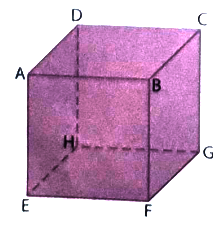
\includegraphics[width=1\linewidth]{6FMA68_imagens/imagem1} \newpage
   			\item No quadriculado abaixo, estão determinados alguns pontos.
   			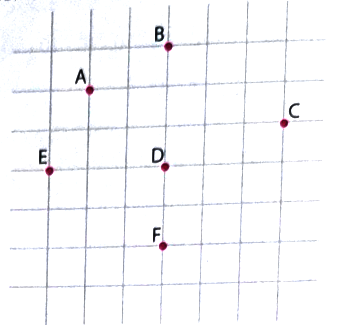
\includegraphics[width=1\linewidth]{6FMA68_imagens/imagem2} \\
   			\begin{enumerate}[a)]
   				\item Trace $\overleftrightarrow{BE}$, $\overleftrightarrow{CF}$, $\overleftrightarrow{DA}$, $\overleftrightarrow{FD}$ e $\overleftrightarrow{EF}$.
   				\item Analise as posições entre as retas desenhadas.
   			\end{enumerate}
   			%72 a 74
	    \end{enumerate} 
        $~$ \\ $~$ \\ $~$ \\ $~$ \\ $~$ \\ $~$ \\ $~$ \\ $~$ \\ $~$ \\ $~$ \\ $~$ \\ $~$ \\ $~$  \\ $~$ \\ $~$ \\ $~$ \\ $~$ \\ $~$ \\ $~$ \\ $~$ \\ $~$ \\ $~$ \\ $~$ \\ $~$ \\ $~$ \\ $~$ \\ $~$ \\ $~$ \\ $~$ \\ $~$ \\ $~$ \\ $~$ \\ $~$ \\ $~$ \\ $~$ \\ $~$ \\ $~$ \\ $~$ \\ $~$ \\ $~$ \\ $~$ \\ $~$ \\ $~$ \\ $~$ \\ $~$ \\ $~$ \\ $~$ \\ $~$ \\ $~$ \\ $~$ \\ $~$ \\ $~$ \\ $~$ \\ $~$ \\ $~$ \\ $~$ \\ $~$ \\ $~$ \\ $~$ \\ $~$ \\ $~$ \\ $~$
	\end{multicols}
\end{document}